\chapter{Introduzione}
\label{chap:intro}

Negli ultimi anni, i sistemi IoT si sono diffusi anche nell'ambito della protezione civile e della gestione delle emergenze, dove la disponibilità di informazioni tempestive e affidabili può incidere direttamente sull'efficacia dei soccorsi.
Il terremoto del 2016 che ha colpito l'Italia centrale, e in particolare l'area di Camerino, ha messo in evidenza questa esigenza. Infatti, nelle prime ore successive a un evento sismico, per i soccorritori è fondamentale sapere dove sono le persone, soprattutto quando potrebbero trovarsi in un luogo difficilmente accessibile o non essere in grado di muoversi. Da qui nasce la domanda alla base della tesi. Quale sensore, tra il PIR a infrarossi passivi e il radar a onde millimetriche (mmWave), rileva la presenza di una persona con maggiore affidabilità?
In questo capitolo vengono presentati gli obbiettivi che hanno guidato il lavoro, insieme a una panoramica della struttura della tesi.

In particolare, la Sezione~\ref{sec:dipme} descrive il progetto DIPME, contesto applicativo del lavoro, la Sezione~\ref{sec:obbiettivo} ne definisce l'obbiettivo e, infine, la Sezione~\ref{sec:struttura} ne illustra l'organizzazione.


\section{Il progetto DIPME}
\label{sec:dipme}

Il confronto tra i due sensori trova uno scenario di applicazione concreto nel progetto DIPME, che ha come obbiettivo la mitigazione del rischio sismico attraverso l'integrazione di sensoristica IoT negli arredi degli ambienti scolastici \cite{slideDipme}. Il progetto costituisce il contesto di riferimento della tesi, che ne riprende il problema e ne valuta una possibile estensione. 
L'idea del progetto si articola su tre livelli:

\begin{itemize}
    \item \textbf{Arredi salva-vita.} Il primo livello riguarda l'arredo stesso. Banchi e pareti sono progettati dalla Scuola di Architettura e Design di UNICAM per resistere al crollo del solaio e mantenere al di sotto di sé un volume in cui una persona possa trovare riparo (Figura~\ref{fig:arredo-render}). Non si tratta quindi di semplici mobili rinforzati, ma di elementi strutturali progettati per lavorare insieme e vincolati tra loro
    \cite{pietroni2021furniture}.

    \item \textbf{Nodi di sensing.} All'interno dell'arredo è integrata l'elettronica della piattaforma DIPME, sviluppata con partner industriali, fra cui AM Microsystems~\cite{slideDipme}, nell'ambito del progetto VITALITY~\cite{callisto2026dipme}. Ogni nodo è un'unità autonoma alimentata a batteria e integra una radio LoRa, un sensore di presenza a infrarossi passivi (PIR) e alcuni sensori ambientali per la misura di temperatura, umidità, pressione e anidride carbonica. I nodi non comunicano
    direttamente con l'esterno, ma con un coordinatore che raccoglie i dati e li inoltra a un gateway locale \cite{callisto2026dipme}.

    \item \textbf{Raccolta e visualizzazione.} Il terzo livello riguarda la raccolta dei dati e la loro visualizzazione. I nodi comunicano via LoRa, che permette di trasmettere a basse potenze anche su distanze dell'ordine di 3--5~km in ambiente urbano. Un gateway locale, alimentato da un gruppo di continuità, coordina il comportamento dei nodi e inoltra i dati a una piattaforma cloud con cruscotti di monitoraggio, conservandoli quando la connessione si interrompe e reinviandoli al ripristino~\cite{callisto2026dipme}. La piattaforma SAFE, di cui DIPME estende l'approccio, prevede inoltre un sottosistema di localizzazione basato su droni e dispositivi mobili a supporto dei soccorritori~\cite{callisto2024safe,callisto2026dipme}.
\end{itemize}

\begin{figure}[htbp]
  \centering
  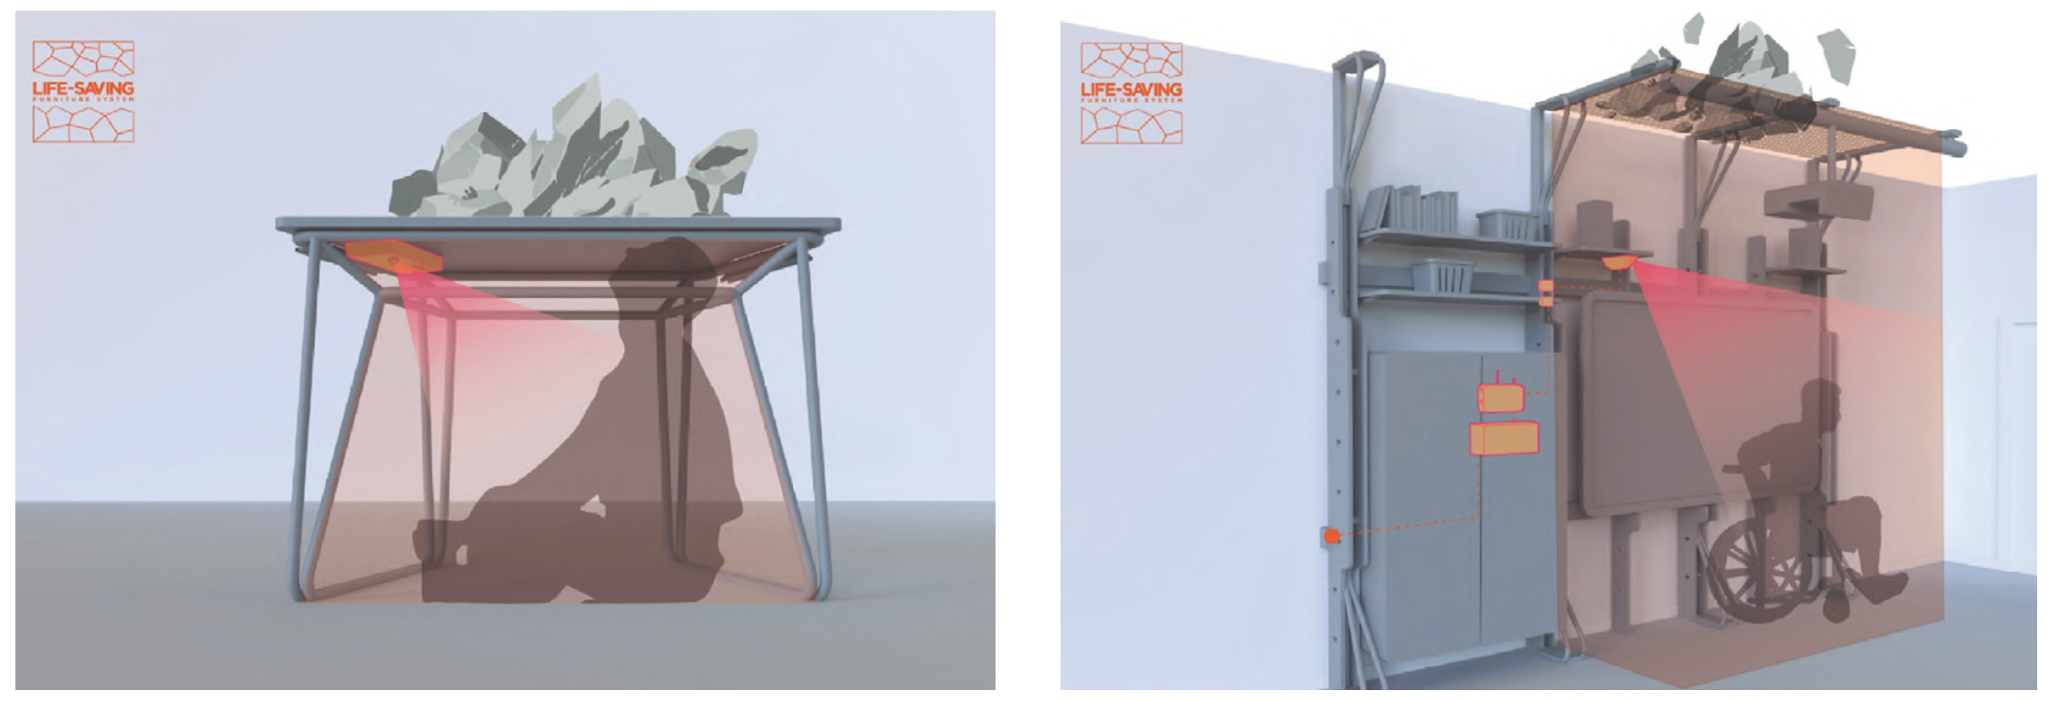
\includegraphics[width=\textwidth]{Immagini/Arredo_salva_vita.png}
  \caption{Il principio dell'arredo salva-vita. Il banco (a sinistra) e la parete attrezzata (a destra) conservano un volume di riparo sotto il carico del crollo. Il nodo di sensing, fissato sotto il piano, osserva l'occupante ~\cite{slideDipme}.}
  \label{fig:arredo-render}
\end{figure}

Il sistema opera in due modalità, un tempo di \emph{pace}, dedicato al monitoraggio ordinario, e un tempo di \emph{guerra}, associato alla gestione dell'emergenza sismica. Il passaggio dalla prima alla seconda è comandato dal gateway al segnale di un accelerometro strutturale. Se il gateway non conferma i messaggi per tre ore, il nodo passa da solo al regime di emergenza. È in questa situazione che il rilevamento della presenza assume un'importanza particolare, perché da questo dato dipende la frequenza con cui il nodo trasmette i propri dati. Se viene rilevata una persona il nodo trasmette un messaggio al minuto, mentre in assenza di presenza la trasmissione avviene ogni quindici minuti. Una persona sotto un banco che il sensore non rileva verrebbe quindi segnalata come assente, e il suo banco trasmetterebbe quindici volte meno spesso, proprio durante l'emergenza. Il dimostratore su cui è stato osservato questo comportamento conta 42 nodi installati nei banchi di due aule di una scuola secondaria delle Marche, in esercizio da ottobre 2025 a marzo 2026 \cite{callisto2026dipme}.

\subsection{Il limite del sensore adottato}
\label{sec:limite-pir}

Il DIPME-DEVICE rileva la presenza attraverso un sensore PIR (Passive InfraRed), la soluzione più diffusa per questa funzione grazie ai consumi e ai costi ridotti. Ha però un limite che non dipende dalla qualità del componente, ma dal suo principio di funzionamento, discusso nel Capitolo~\ref{chap:sensori}. Il sensore risponde infatti alla variazione del flusso infrarosso, non al suo valore, e quindi non è in grado di rilevare una persona immobile. 

Nello scenario DIPME questo limite si presenta proprio nella situazione più critica, perché una persona rifugiata sotto un banco dopo un crollo è, tipicamente, ferma. Gli stessi autori della piattaforma indicano, tra gli sviluppi futuri, l'estensione del sistema di sensing con radar a onde millimetriche a complemento del PIR, da valutare in termini di accuratezza, consumo, privacy e complessità \cite{callisto2026dipme}. 

I radar mmWave a 24 GHz promettono di superare questo limite grazie alla capacità di rilevare i micro-movimenti e di misurare la distanza del bersaglio.


\section{Obbiettivo}
\label{sec:obbiettivo}

La tesi si propone di confrontare sperimentalmente due tecnologie di rilevamento di presenza, il sensore PIR e il radar mmWave a 24 GHz. L'obbiettivo è stabilire, attraverso misure ripetibili, quale delle due rilevi la presenza di una persona con maggiore affidabilità in uno scenario post-sisma, e quanto sia ampio il divario tra loro. Il caso di riferimento è quello della persona immobile sotto un arredo. Il risultato interessa direttamente il progetto DIPME, il cui nodo affida oggi il rilevamento al solo PIR.

Il lavoro è stato organizzato in sei punti:

\begin{itemize}
    \item \textbf{O1. Studiare i sensori}, per capire chi li utilizza, in quali contesti e quali dati producono.

    \item \textbf{O2. Analizzare i dati forniti}, per capire quali grandezze ciascun sensore mette a disposizione e con quale accuratezza.

    \item \textbf{O3. Confrontare sperimentalmente} PIR e mmWave con metriche quantitative.

    \item \textbf{O4. Valutare il consumo energetico}, a titolo informativo e sulla base dei datasheet, non essendo disponibile la strumentazione per misurarlo.

    \item \textbf{O5. Realizzare un'interfaccia web} che mostri i dati in tempo reale, li salvi e li esporti in formato CSV per l'analisi numerica.

    \item \textbf{O6. Definire un indice di vitalità} che, oltre alla presenza, misuri quanto una persona si muove.
\end{itemize}

Gli altri elementi del progetto DIPME (la radio LoRa, il gateway, la piattaforma cloud e il Digital Twin) e il sottosistema di localizzazione con i droni della piattaforma SAFE non sono oggetto della tesi e compaiono nella Sezione~\ref{sec:dipme} solo per inquadrare il contesto in cui il confronto trova applicazione.

\section{Struttura della Tesi}
\label{sec:struttura}

\begin{itemize}
    \item \textbf{Sensori di presenza: principi e stato dell'arte.} Il Capitolo~\ref{chap:sensori} spiega come funzionano il PIR e il radar FMCW a onde millimetriche e li colloca rispetto alle alternative (O1).
    
    \item \textbf{I moduli in esame e i dati che producono.} Il Capitolo~\ref{chap:moduli} presenta i tre sensori impiegati a partire dalla documentazione ufficiale, e la piattaforma di acquisizione su ESP32 con il formato dati comune a tutta la tesi (O2).
    
    \item \textbf{Metodologia di confronto.} Il Capitolo~\ref{chap:metodologia} fissa il protocollo, le metriche e le convenzioni con cui i sensori sono stati confrontati, e presenta l'interfaccia web servita direttamente dall'ESP32, senza alcuna rete esterna, realizzata a supporto della campagna (O5).

    \item \textbf{Confronto sperimentale.} Il Capitolo~\ref{chap:confronto} è il capitolo centrale e raccoglie i risultati della campagna di misura, con ogni risultato accompagnato dalla sua dispersione su ripetizioni indipendenti (O3).

    \item \textbf{Indice di vitalità.} Il Capitolo~\ref{chap:vitalita} misura il respiro con verifica a ritmo imposto, poi definisce, tara e valida l'indice e ne descrive il porting a bordo del microcontrollore (O6).

    \item \textbf{Consumo energetico.} Il Capitolo~\ref{chap:consumi} stima consumi e autonomia dei tre sensori e discute l'architettura ibrida PIR + mmWave che ne discende (O4).

    \item \textbf{Conclusioni e sviluppi futuri.} Il Capitolo~\ref{chap:conclusioni} risponde alla domanda di partenza, dichiara i limiti del lavoro e indica come proseguirlo.
\end{itemize}